\section{Tell Me Something New}\label{sec:tmsn}
We start with a general description of \tmsn\ which will be followed
by a description of \tmsn\ for boosting.

Many learning algorithms can be described as {\em loss
  minimizing}. The goal of such algorithm is to find a model that
minimizes some loss function on the training data.  Loss minimizing
algorithms often operate {\em incrementally}. Here are a few examples:
Each step in a {\em stochastic gradient descent} algorithm corresponds
to an update step of the parameters that decreases the loss on a
single example. A {\em tree learning algorithm} repeatedly identifies
which leaf to split so as to minimize an ``impurity'' function. A {\em 
  Boosting} algorithm finds a weak rule that minimizes the
classification error with respect to a weighted sample.

The goal of a loss minimizing algorithm is to minimize the {\em true
  expected loss} with respect to the underlying distribution. However,
the algorithm cannot minimize the expected loss directly, instead, it
minimizes the {\em empirical loss} measured with respect to the
training set. The difference between the training loss and the test
loss is the {\em overfit} which decreases as the size of the training
set increases. This leads to a natural tradeoff between run-time and
the amount of overfit. A larger training set gives more accurate
estimates but longer running time and vice versa.

One example of this tradeoff is the different types of gradient
descent. At one extreme, batch gradient descent computes the gradient
using all of the training data and then makes an update step. At the
other extreme, SGD makes an update step after reading each
example. Mini-batch SGD lies in the middle, where an update is
performed after each mini-batch. Experience has shown that SGD
converges fater than batch gradient descent is useful in parallelized
SGD.

In this paper we describe a novel approach to balancing compute-time
and accuracy. Our algorithm computes, in addition to the estimate of
the loss, an estimate of the {\em error} in the loss estimate. When
this error estimate is sufficiently small, the algorith stops reading
data and uses the current estimate.

We call this approach to machine learning ``tell me something new'' or
\tmsn. In the next section we provide a general theory for \tmsn.

We denote a model by $M$, a randomly selected datapoint
by $\vx$\footnote{The \tmsn\ framework can be applied to both
  supervised and unsupervised learning.} and the loss associated with
model $M$ applied to the example $\vx$ by $L(M,\vx)$. Using this
notation 
$\vec{x}$ 
To streamline our presentation
we consider binary classification, but other supervised or
unsupervised learning problem can be accommodated with little change.

We are given
\newcommand{\cD}{{\cal D}}
\begin{itemize}
\item A set of classifiers $\strongRules$, each classifier $H \in
  \strongRules$ is a mapping from an input space $X$ to a binary label $\{-1,+1\}$.
\item A stream of labeled examples $(x_1,y_1),(x_2,y_2),\ldots$, $x_i
  \in X$, $y_i \in \{-1,+1\}$, generated IID according to a fixed but
  unknown distribution $\cD$.
\end{itemize}

The goal of the algorithm is to find a classifier $H \in
\strongRules$ that minimized the error probability $\err(H)\doteq
P_{(x,y) \sim \cD}[H(x) \neq y]$

All workers start from the same initial classifier $H_0$ which is
improved iteratively. Some iterations end with the worker finding a
better classifier by itself, others end with the worker receiving a
better classifier from another worker. The sequences of classifiers
corresponding to different workers can be different, but with high
probability they all converge to the same classifier.

Denote each worker by an index $i=1,\ldots,n$. On iteration $t$
each worker has its {\em current} classifier  $H_i(t)$ and a set of $m$
{\em candidate} classifiers $G_i^j(t)$. An error upper bound
$\errub(H_i(t))$ is associated with $H_i(t)$ so that with high
probability $\errub(H_i(t)) \geq \err(H_i(t))$.

\begin{figure}[t]
%\begin{minipage}{.31\textwidth}
\begin{center}
  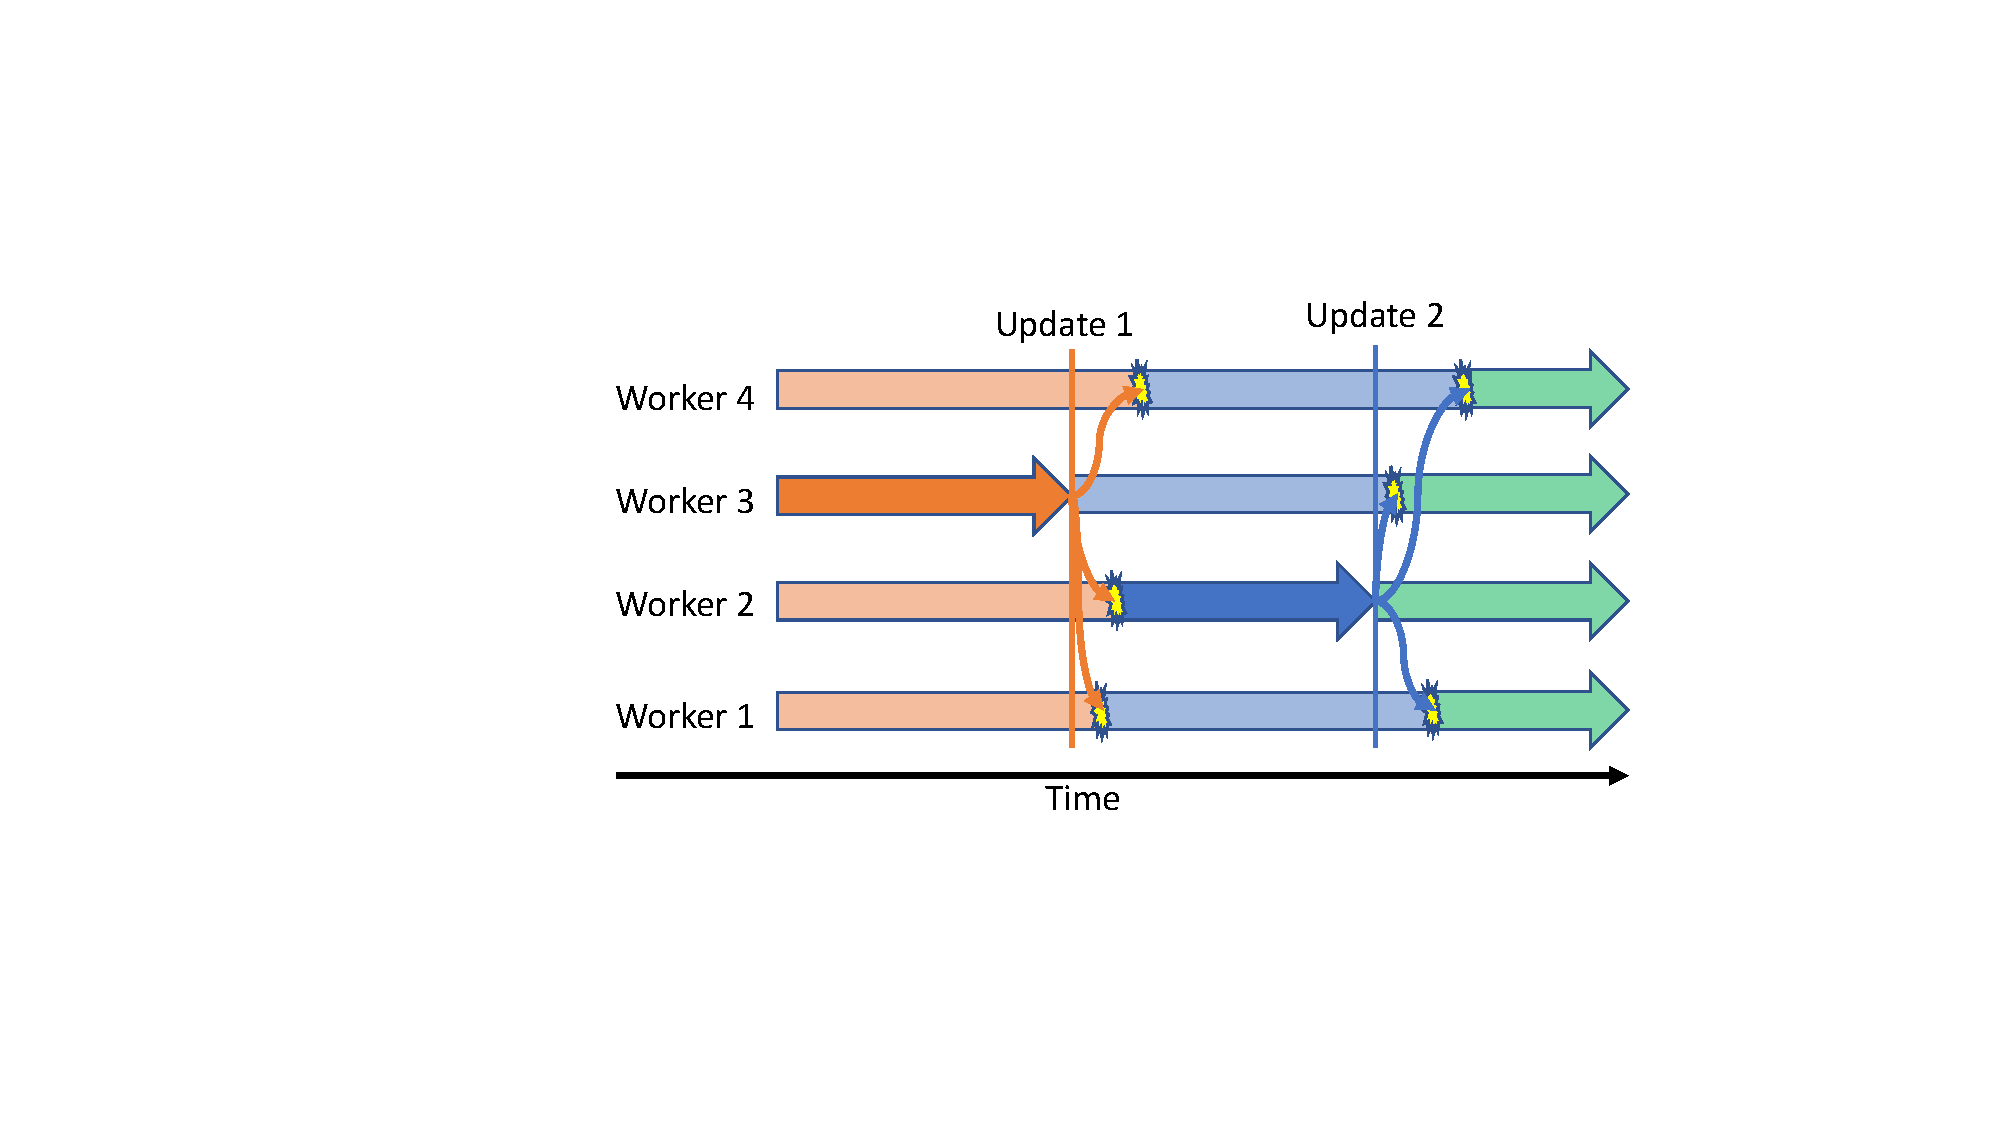
\includegraphics[width=0.7\textwidth]{AsyncUpdates.pdf}
\end{center}
  \caption{{\bf Execution timeline of a \tmsn\ system}
      System consists of four workers. The first update occurs when
      worker 3 identifies a better classifier $H_1$. It then replaces
      $H_0$ with $H_1$ and broadcasts $(H_1,z_1)$ to the
    other workers. The other workers receive the message the at different
    times, depending on network congestion. At that time they  interrupt the
    scanner (yellow explosions) and start using $H_1$. Next, worker 2
    identifies an improved rule $H_2$ and the same process ensues.
    \label{fig:async}}
   	\vspace{0pt}
%\end{minipage}
\end{figure}

The worker reads examples from the stream and uses them to estimate
the errors of the candidates. It stops when it finds a candidate that,
with high probability, has an error smaller than
$\errub(H_i(t))-\epsilon$ for some constant ``gap'' parameter
$\epsilon>0$.

More precisely, the worker uses a {\em stopping rule} that chooses a
stopping time and a candidate rule and has the property that, with
high probability, the chosen candidate rule has an error smaller than
$\errub(H_i(t))-\epsilon$. This candidate then replaces the current
classifier, the new upper bound is set to be $\errub(H_i(t+1)) =
\errub(H_i(t))-\epsilon$, a new set of candidates is chosen and the
worker proceeds to the next iteration. At the same time the worker
{\em broadcasts} the pair $(H_i(t+1), \errub(H_i(t+1))$.

A separate process in each worker listens to broadcasts of this
type. When worker $i$ receives a pair $(H,\errub(H))$ it compares the
upper bound $\errub(H)$ with the upper bound associated with it's
current classifier $\errub(h_i(t))$. If $\errub(H) < \errub(h_i(t))-\epsilon$,
it interrupts the current search and sets $H_i(t+1)=H$. If not the
received pair is discarded.

Note that the only assumption that the workers make regarding the
incoming messages is that the upper bound $\errub(H)$ is sound. In
other words that, with hight probability, it is an upper bound on the
true error $\err(H)$. There is no synchronization and if a worker is
slow or fails, the effect on the other workers is minimal.

Different implementations of \tmsn\ differ in the way that they
generate candidate classifiers and in the stopping rules that they
use. For \tmsn\ to be effective, the stopping rule should be both
sound and tight. If it is not sound, then the scheme falls apart, and
if it is not tight, then the stopping rules stop later than needed,
slowing down convergence.

Next, we describe how \tmsn\ is applied to boosting.
